\chapter{Introduction}
\epigraph{\small\itshape ``Progress in science depends on new techniques, new discoveries and new ideas, probably in that order.''}{\small\textit{---Sidney Brenner}}

Understanding the human brain is one of the most significant challenges of the 21st century. The human brain is arguably one of the most important organs of the human body, which performs a wide range of cognitive functions: from visual recognition to language understanding, speech, social interaction, and executive control. Even then, pathologies of the brain are perhaps on of the biggest challenges for western medicine today. Medical interventions and drugs for major infectious diseases are available today, and individuals can expect to live up to the mid 80s and even into their 90s. Yet, we still do not have a grasp over most mental pathologies: Parkinson's, Alzheimer's, dementia, epilepsy to name a few. The scale of the problem is enormous. Today, a person living into their mid 80s has a 50\% chance of contracting Alzheimer's~\citep{alzheimer20162016}.

Our current understanding of the brain is a result of decades of concerted efforts across multiple disciplines ranging from molecular biology, genetics, physiology, cognitive and behavioral neuroscience, to statistics and computer science.

After a brief introduction to modern brain imaging, I will outline four areas of ... and how this thesis progresses the state-of-the-art:
 
\section{Modern brain imaging}
Brain imaging tools today can be placed along three axes: their temporal resolution, their spatial resolution, and the level to which they are invasive.

\begin{figure}[htb]
\begin{center}
   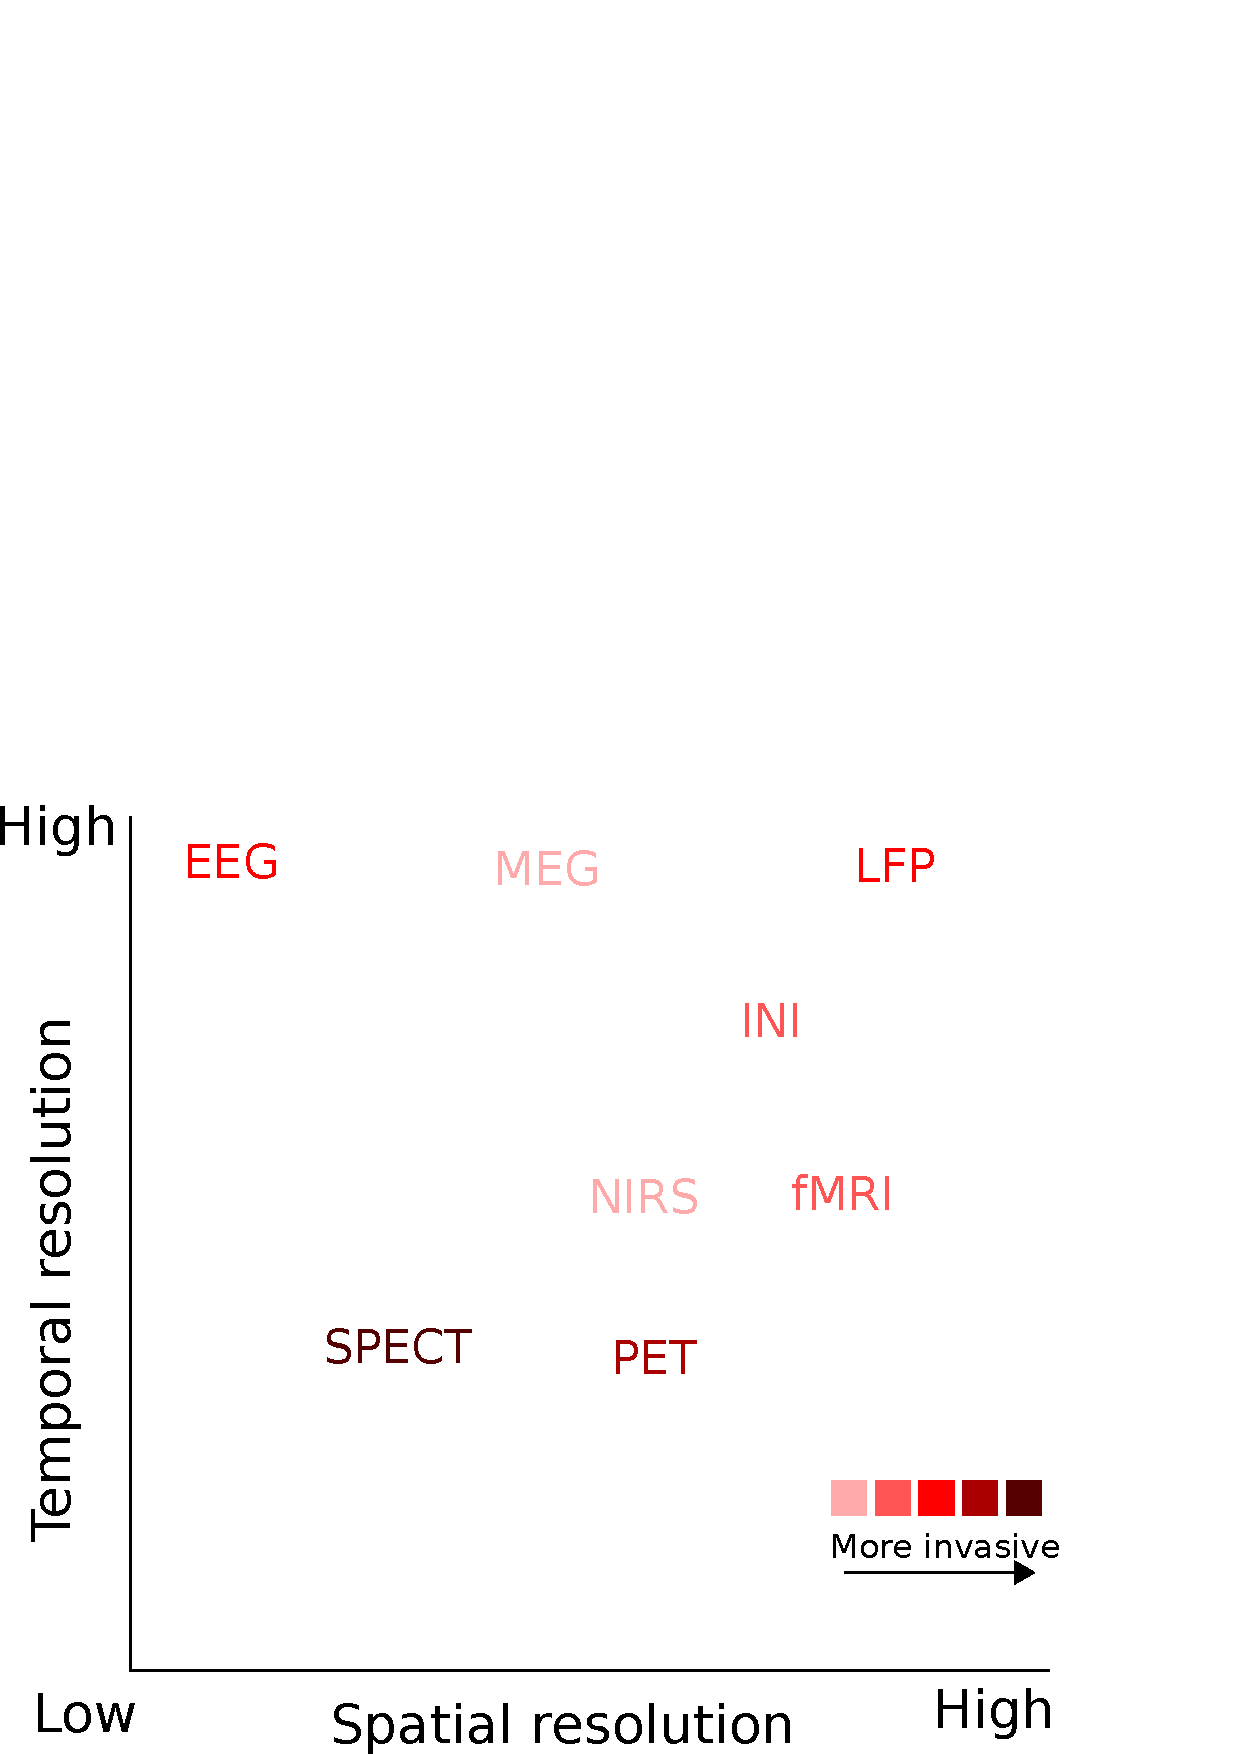
\includegraphics[width=0.4\linewidth]{figures/neuroimaging_methods.pdf}
\end{center}
   \caption[Various neuroimaging methods differ in terms of the information they measure.]{Various neuroimaging methods differ in terms of the information they measure. MEG=magnetoencephalography, EEG=electroencephalography, NIRS=near-infrared spectroscopy, PET=positron emission tomography, SPECT=single photon emission tomography, and INI=Inverse imaging, a method to speed up acquisition of fMRI images.}
   \label{fig:neuroimaging_methods}
\end{figure}

\clearpage
\section{The reproducibility crisis}

Even though thousands of papers are published every year about different aspects of the brain, our understanding of this complex organ has not scaled in proportion. A large part of the reason has been attributed to what is known as the reproducibility crisis~\citep{ioannidis2005most, simmons2011false, button2013power}. %Replication is closely related to the concept of reproducibility which refers to the idea that an experiment produces the same result when performed again under the same conditions. Replication is a stronger condition as it requires similar results or identical conclusion even if there are some minor variations in the experimental procedures. 
Progress in science rests on reproducible experiments. In many fields, however, a large fraction of experiments cannot be reproduced. In psychology, for instance, it was estimated that over half of the papers were not reproducible~\citep{open2015estimating}, and even those which could be reproduced tended to have a weaker effect size compared to the original study. The reasons for unreproducible results can be many, some being: 1) confirmation bias, the tendency to selectively report only experiments that conform to the researcher's pre-existing beliefs, 2) ``p-hacking''~\citep{simmons2011false}, or the tendency to try multiple hypothesis to get a positive result, 3) publication bias or the absence of incentives to publish negative results, and 4) pressure to publish. There are now an accepted set of recommendations to counter many of these issues: 1) pre-registering research plans to avoid confirmation bias and even report negative results, 2) correct for multiple comparisons, the most conservative method being the Bonferroni correction [ref]. 

However, brain imaging has its own set of unique issues which can be linked to reproducibility crisis: 

% vul2009puzzlingly
% yendiki2014spurious

\begin{itemize}[noitemsep,partopsep=0pt]
\item \textbf{Multiple comparison:} Same as in the case of psychology but more widespread due to the presence of large number of voxels or time points [ref]. For instance, in the famous dead salmon study~\citep{bennett2009neural}, an effect was found even if none was expected.
\item \textbf{Differences in software versions:} For instance in the case of Freesurfer software [ref], it can lead to almost a 1 mm [check] difference in cortical thickness~\citep{gronenschild2012effects}.
\item \textbf{Complex pipelines:} Neuroimaging pipelines involve a number of choices at each processing stage, and there isn't currently a consensus on how to choose the right pipeline. Often, these methodological choices are not even documented. It is estimated that almost every new study has its own unique pipeline~\citep{Carp2012289}.
\item \textbf{Power failure:} This is arguably one of the central issues in the reproducibility crisis today and has received by far the most attention. The statistical power of a study refers to the likelihood of discovering an effect of interest, given the sample size. Small sample sizes translate into underpowered studies which means that the chance of a false discovery is high. In order to discover the effect of interest, the study must be appropriately powered. This is closely related to the problem of multiple comparisons as it is more prevelant in underpowered studies.
\item \textbf{Methodological concerns:} There are several methodological concerns, but perhaps one that has received some attention is the issue of head movements~\citep{yendiki2014spurious} which can lead to spurious correlations.
\end{itemize}

The issue of complex pipelines will be revisited in Chapter~\ref{chapter:group_study} as we provide concrete guidelines on how to select the appropriate pipeline. For now, let us turn our attention to data sharing which can help us alleviate the issue of power failure.

\clearpage
\section{Data sharing}
The history of data sharing can be traced back to Newton and his theory of gravitation~\citep{pointofview2013}. Before Newton had developed his theory, another English astronomer, John Flamsteed had been appointed by the king to observe the stars and produce accurate charts for navigation in the seas. Over a period of 40 years, Flamsteed created a detailed catalogue that tripled the number of entries in the previously used sky atlas. When the great comet of 1680 appeared in the sky twice in close succession, Flamsteed used his data to postulate that it was not two comets but in fact the same comet which first went towards the sun and then turned away from it. Newton initially opposed this theory, but later changed his mind as he gained access to Flamsteed's unpublished catalogue. The comet had indeed turned out to be an important benchmark for Newton's theory of gravitation.

It is hard to imagine in this day and age that a theory as fundamental as the laws of gravitation could have been data driven. Today, data sharing is fundamental to reproducible science, but it also forms the cornerstone for learning better models and benchmarking new algorithms. If one follows the breakthroughs in the field of machine learning, for instance, it is predicated on the availability of data. It is an almost undisputed fact that the recent resurgence of deep learning owes in part at least, to the release of Imagenet~\citep{deng2009imagenet}. The same is true for Q learning in Atari games~\citep{watkins1992q, bellemare2013arcade}, natural language processing for language translation [ref], speech recognition [ref], and even the mixture of experts model~\citep{jacobs1991adaptive} for IBM Watson~\citep{ferrucci2010building}. If such datasets were available in neuroscience, we would be able to tease apart even subtle effects that were not possible before with smaller sample sizes.

Of course, neuroscientists are beginning to realize the importance of sharing data. In recent times, neural data has started being shared through international consortiums~\citep{van2013wu, ollier2005uk} and data repositories~\citep{poldrack2013toward, gorgolewski2015neurovault}. While in the case of Newton, he gained access to the catalogue without permission, today it is possible to publish dataset papers in targeted journals so as to assign the credit where it is due.
Data sharing is beneficial not just from the perspective of replication but also from an economic perspective. Rather than collect new data for every new hypothesis, researchers can now reuse existing data for answering their hypotheses.

\subsection{Brain Imaging Data Structure}

\clearpage
\section{Automation}
Back in 2014, Nature published a bold article~\citep{hayden2014automated} which described a vision for the future of science: ``solving the problem of bringing McDonald's-like efficiency to scientists''. This would in turn lead to cheaper, more efficient and reliable research. While it goes on to describe many biology labs which are automating experiments, the benefits of automation in the neuroimaging community are yet to be widely recognized. Automation not only saves time but also makes the research more reproducible, as was noted in a recent guide to improve the transparency and reproducibility of neuroimaging research~\citep{gorgolewski2016practical}. The authors point out that manual work may seem easy at first, if the analysis has to be performed only once. However, this is not always the case as ``quite often in the course of a project, parameters are modified, subjects are changed, and processing steps need to be rerun. This is a situation in which having a set of scripts that can perform all of the processing steps automatically instead of relying on manual interventions can really pay off.''

Let us consider some of the opportunities for automation in neuroimaging:
\begin{itemize}[noitemsep,nolistsep,nosep]
\item \textbf{Reducing interactivity:} While interactive graphical user interfaces are excellent tools for browsing the data, they fall short when it comes to scaling the analysis, which is necessary for a sufficiently powered study. 

\item \textbf{Parameter tuning:} Most algorithms, although scripted, still require hyperparameters to be tuned. These hyperparameters could be the number of ICA components to choose or the regularization parameters, and can vary for each subject.
%This could be the number of trials to perform in an experiment, the number of components to select in a \ac{PCA} decomposition, or the regularization parameter in inverse solvers.
\item \textbf{Annotation and labeling:} A large fraction of neuroimaging data that is available is unlabeled or at best weakly labeled. This is because expert annotations are expensive, and cannot be crowdsourced. Automated tools based on unsupervised learning can play a major role in this regard.
\item \textbf{Quality control:} Currently, quality control is performed manually by inspecting the data to spot outliers. While data inspection cannot be overlooked, it can be performed more efficiently through automated documentation of data analysis and log reports such as the Jupyter notebook and the MNE web report. At the same time, advanced statistical trend analyses as in the Automated Statistician project~\citep{duvenaud2013structure} can be used for creating summaries.
\end{itemize}
In this thesis, we will consider an algorithm for automated artifact rejection~\citep{jas2016automated, jas2017autoreject}. This is a first step that any M/EEG processing pipeline has to go through but it is often done manually. The reason for this is that existing algorithms are not designed to be \emph{transparency}. Since for more scientists, the key to new insights is an artifact-free dataset, they would rather spend some extra time in doing this manually rather than depend on a generic algorithm which is difficult to interpret. However, this is problematic as it can lead to a selection bias: they might end up rejecting data segments which helps them confirm their hypothesis. Merely based on anecdotal reports, this process can take up to a week even for a moderately sized study of 10--20 subjects.

This is what led us to propose \emph{autoreject}, which we describe in Chapter~\ref{chapter:autoreject}. It is an algorithm which can be used to mark bad segments of the data. The key insight is that, often certain sensors in the device are intermittently corrupted rather than continuously. We validate our algorithm against 3 benchmarks on the HCP dataset~\citep{larson2013adding} which is manually annotated with bad segments.

% automated statistician
%
% This subjectivity can lead to studies which are not reproducible unless every single detail was carefully documented. Even then, it does not rule out a potential confirmation bias: the tendency to favor processing steps which leads one to confirm the hypothesis being tested rather than reject it.

\clearpage
\section{Representation learning}
In the last 100 years since the invention of EEG, scientists have discovered several different brain oscillation patterns such as alpha waves, K-complexes, and mu rhythms. The oscillations and interactions between them have served as biomarkers for different brain functions and pathologies. Alpha waves have been implicated in attention, K-complexes in sleep, and mu rhythm in motor activity. 

Considering the complexity of the human brain, clearly these waveforms represent only a fraction of the cognitive functions that the brain may perform. As a result of the wealth of data now available through the data sharing movement described in Section~\ref{chapter:alphacsc}, the future neuroscientist will be able to mine such waveforms from large datasets. Imagine if neuroscientists had at their disposal a tool similar to Google Photos\footnote{\url{https://photos.google.com/}}. Rather than automatically finding faces and grouping photos, it would find prototypical oscillations and cluster the data using them. Clicking on any of these waveforms would retrieve the data associated with them.

\begin{figure}[htb]
\begin{center}
   \includegraphics[width=0.7\linewidth]{figures/schema.pdf}
\end{center}
   \caption[Convolutional sparse coding]{Convolutional sparse coding}
   \label{fig:neuroimaging_methods}
\end{figure}

However, photos are inherently different from neural data. First, neural data can be buried in noise and corrupted by high amplitude artifacts. Second, images are labelled due to datasets such as Imagenet [], but neural data is not. Finally, it is spatiotemporal data with different dynamics than the 3D world that photos capture. This is where convolutional sparse coding (CSC) can play a role by extracting prototypical features from the data. It is an unsupervised algorithm from computer vision, which can learn shift-invariant representations from the data using convolutional operations.

Current efforts in extracting known waveforms capitalize on heavy signal processing based on the Fourier transform. This involves approximating the waveform by a sinusoidal basis

However, as these waveforms are buried in the noise, extracting them would require heavy signal processing techniques, particularly those based on Fourier transforms, to emphasize the signal of interest. Obviously, this is not ideal as the sinusoidal bases offered by Fourier transform is not the most compact. A square wave for instance would need to be approximated by a infinite series of sinusoids. Wavelets have therefore been suggested to model the transients. Yet, sinusoidals and wavelets are at best approximations. To best preserve the shape of the waveform, it is necessary to learn the waveform directly from the data. This is the aspiration of representation learning.

In our work, we focus on dictionary learning, a representation learning technique that allows us to learn prototypical `atoms' and their corresponding `activation' maps. As data sharing increases, such a technology is likely to be indispensable as it will allow mining prototypical waveforms on large datasets.

\clearpage
\section{Contributions}
In this thesis, I attempt to synthesize the lessons learned from analysing public neuroimaging data with open source software. To this effect, I participated in an effort to create an MEG standard for the Brain Imaging Data Structure (BIDS)~\citep{galan2017meg}. I wrote the validator which helped create the MEG-BIDS compatible example datasets. As a contributor to MNE~\citep{gramfort2013meg}, I led an effort to write a tutorial paper which reanalyzes the Faces dataset~\citep{wakeman2015multi} for a reproducible group study. This led us to develop a fully automated algorithm for artifact rejection and repair~\citep{jas2016automated, jas2017autoreject}. Finally, we develop algorithms to learn new undiscovered motifs automatically from neural time series data. 

\subsection*{Journal publications}
\bibentry{jas2017autoreject} \\ \\
\bibentry{jas2017mne} \\ \\
\bibentry{galan2017meg}

\subsection*{Conference publications}
\bibentry{jas2016automated} \\ \\
\bibentry{jas2017learning}